\documentclass[aps,prl,twocolumn,superscriptaddress]{revtex4-2}
\usepackage{graphicx}
\usepackage{amsmath}
\usepackage{amssymb}
\usepackage{tikz}
\usepackage{pgfplots}
\pgfplotsset{compat=1.18}
\usepackage{listings}
\usepackage{xcolor}
\usepackage{fancyhdr}
\usepackage{xurl} % for better url line breaking
\usepackage[hidelinks]{hyperref} % for hyperlinks

% Header & Footer configuration
\pagestyle{fancy}
\fancyhf{}
\fancyhead[L]{A.T. Azza'im}
\fancyhead[R]{Random Walk Klasik dan Quantum Walk}
\renewcommand{\thesection}{\Roman{section}}
\setcounter{secnumdepth}{3}
\renewcommand{\headrulewidth}{0.4pt}
\fancyfoot[C]{\thepage}
\fancypagestyle{plain}{
    \fancyhf{}
    \renewcommand{\headrulewidth}{0pt}
    \fancyfoot[C]{\thepage}
}

% Code snippet configuration (Jupyter Notebook style)
\lstdefinestyle{jupyter}{
    backgroundcolor=\color{gray!10},
    commentstyle=\color{green!50!black},
    keywordstyle=\color{blue},
    numberstyle=\tiny\color{gray},
    stringstyle=\color{red},
    basicstyle=\ttfamily\footnotesize,
    numbers=left,
    numbersep=8pt,
    breaklines=true,
    frame=single,
    language=Python
}

\begin{document}

\title{Perbandingan Random Walk Klasik dan Quantum Walk}
\author{\textbf{Akmal Taqiyyuddin Azza'im}\\
    \normalsize Program Studi Magister Fisika, Departemen Fisika, Fakultas Matematika dan Ilmu Pengetahuan Alam, Universitas Gadjah Mada\\}
\maketitle

\section{Pendahuluan}

    \subsection{Latar Belakang}

        Getaran transversal pada senar yang tegang dapat dimodelkan
        menggunakan persamaan gelombang satu dimensi dengan parameter
        fisis berupa massa jenis linear dan tegangan senar
        \cite{BillinghamKing2000}. Karakteristik getaran senar dapat
        diinvestigasi melalui analisis frekuensi rekaman suara menggunakan
        Transformasi Fourier Cepat (\textit{Fast Fourier Transform},
        FFT). Penggunaan fungsi jendela dalam analisis spektrum diperlukan
        untuk mengurangi pengaruh pemotongan sinyal terhadap hasil
        transformasi \cite{Harris1978}.

        Persamaan gelombang kemudian diselesaikan menggunakan metode
        beda hingga, yaitu dengan mendiskretisasi turunan ruang dan
        waktu pada domain komputasi. Keakuratan metode dievaluasi melalui
        pengujian kestabilan dan konvergensi, sedangkan pengembangan
        model dengan suku redaman digunakan untuk menginvestigasi
        perubahan dinamika dan energi gelombang
        \cite{LeVeque2007}.

    \subsection{Tujuan}

        Pekerjaan ini bertujuan untuk:
        \begin{enumerate}
            \item Mengestimasi frekuensi fundamental dan parameter fisis
            senar gitar berdasarkan pengukuran serta analisis rekaman audio.

            \item Mengimplementasikan metode beda hingga untuk
            menyelesaikan persamaan gelombang satu dimensi serta
            mengevaluasi kestabilan dan konvergensi solusi numerik.

            \item Menganalisis pengaruh redaman terhadap evolusi gelombang
            dan perubahan energi sistem.
        \end{enumerate}

\section{Model Fisis dan Parameter Senar}
\label{sec:model-fisis}

    \subsection{Model Gelombang pada Senar Ideal}

        Getaran transversal pada senar ideal yang tegang dapat dimodelkan menggunakan persamaan gelombang satu dimensi \cite{BillinghamKing2000}. 
        Dengan mengabaikan pengaruh redaman dan kekakuan senar, persamaan geraknya dinyatakan sebagai
        \begin{equation}
            \frac{\partial^2 y}{\partial t^2} = c^2 \frac{\partial^2 y}{\partial x^2},
            \label{eq:wave-equation}
        \end{equation}

        dengan $y(x,t)$ merupakan simpangan transversal senar, $c$ adalah cepat rambat gelombang, dan $x$ serta $t$ masing-masing menyatakan posisi dan waktu. 
        
        Cepat rambat gelombang pada senar ditentukan oleh
        \begin{equation}
            c = \sqrt{\frac{T}{\mu}},
            \label{eq:wave-speed}
        \end{equation}
        dengan $T$ merupakan tegangan senar dan $\mu$ adalah massa jenis linear senar.
        Untuk senar dengan kedua ujung terikat, frekuensi fundamental memenuhi hubungan
        \begin{equation}
            f_1 = \frac{c}{2L},
            \label{eq:fundamental-frequency}
        \end{equation}
        sehingga cepat rambat gelombang dapat diestimasi melalui
        \begin{equation}
            c = 2Lf_1.
            \label{eq:wave-speed-estimation}
        \end{equation}

    \subsection{Model Gelombang dengan Redaman}

        Pada senar nyata, sebagian energi mekanik dapat terdisipasi akibat mekanisme redaman. 
        Pengaruh tersebut dimodelkan dengan menambahkan suku yang sebanding dengan kecepatan transversal senar. 
        Persamaan gelombang teredam dituliskan sebagai
        \begin{equation}
            \frac{\partial^2 y}{\partial t^2} + \gamma \frac{\partial y}{\partial t} = c^2 \frac{\partial^2 y}{\partial x^2},
            \label{eq:damped-wave-equation}
        \end{equation}
        dengan $\gamma$ merupakan koefisien redaman yang memiliki satuan $\mathrm{s}^{-1}$. 
        Ketika $\gamma=0$, persamaan tersebut kembali menjadi persamaan gelombang tanpa redaman.

    \subsection{Kondisi Awal dan Kondisi Batas}

        Domain senar didefinisikan pada interval $0\leq x\leq L$.
        Kedua ujung senar dianggap terikat sehingga memenuhi kondisi batas tetap,
        \begin{equation}
            y(0,t)=y(L,t)=0.
            \label{eq:boundary-condition}
        \end{equation}
        Simulasi dimulai dari profil simpangan awal berbentuk segitiga dengan amplitudo maksimum $h$ pada posisi $x=x_p$. 
        Profil tersebut dinyatakan sebagai
        \begin{equation}
            y(x,0)=f(x)=
            \begin{cases}
                h\displaystyle\frac{x}{x_p},
                & 0\leq x\leq x_p, \\[8pt]
                h\displaystyle\frac{L-x}{L-x_p},
                & x_p < x\leq L.
            \end{cases}
            \label{eq:initial-profile}
        \end{equation}
        Senar diasumsikan dilepaskan dari keadaan diam sehingga kecepatan transversal awal bernilai nol,
        \begin{equation}
            \left.\frac{\partial y}{\partial t}\right|_{t=0}
            =0.
            \label{eq:initial-velocity}
        \end{equation}
        Profil awal segitiga digunakan untuk merepresentasikan simpangan senar setelah diberi petikan. 
        Dalam simulasi, amplitudo awal ditetapkan sebesar $h=10^{-3}\,\mathrm{m}$.

    \subsection{Estimasi Parameter Fisis Senar}

    Parameter fisis senar ditentukan berdasarkan panjang senar, frekuensi fundamental hasil analisis rekaman audio, serta estimasi massa senar. 
    Massa jenis linear dihitung menggunakan
    \begin{equation}
        \mu = \frac{m}{L},
        \label{eq:linear-density}
    \end{equation}
    sedangkan tegangan senar diperoleh dengan menggabungkan Persamaan~\eqref{eq:wave-speed} dan Persamaan~\eqref{eq:wave-speed-estimation}, yaitu
    \begin{equation}
        T = \mu(2Lf_1)^2.
        \label{eq:string-tension}
    \end{equation}
    Panjang bebas senar hasil pengukuran adalah $L=(0{,}658\pm0{,}001)\,\mathrm{m}$. 
    Frekuensi fundamental diperoleh dari rata-rata tiga pengukuran petikan. 
    Massa senar tidak diukur secara langsung, melainkan diasumsikan sebesar $22{,}5\,\mathrm{g}$ untuk panjang senar tersebut, dengan rentang asumsi $22$--$23\,\mathrm{g}$.
    Dengan menggunakan parameter tersebut, diperoleh estimasi besaran fisis sebagaimana ditunjukkan pada Tabel~\ref{tab:physical-parameters}.

    \begin{table}[htbp]
        \centering
        \caption{Estimasi parameter fisis senar gitar.}
        \label{tab:physical-parameters}
        \begin{tabular}{lll}
            \hline
            Besaran & Nilai & Keterangan \\
            \hline
            $L$ &
            $(0{,}658\pm0{,}001)\,\mathrm{m}$ &
            Pengukuran \\

            $f_1$ &
            $328{,}501\,\mathrm{Hz}$ &
            Rata-rata tiga petikan \\

            $m$ &
            $(22{,}50\pm0{,}29)\,\mathrm{g}$ &
            Asumsi \\

            $\mu$ &
            $(0{,}03419\pm0{,}00044)\,\mathrm{kg/m}$ &
            Hasil perhitungan \\

            $c$ &
            $(432{,}31\pm0{,}66)\,\mathrm{m/s}$ &
            Hasil perhitungan \\

            $T$ &
            $(6{,}391\pm0{,}083)\times10^3\,\mathrm{N}$ &
            Hasil perhitungan \\
            \hline
        \end{tabular}
    \end{table}

    Ketidakpastian massa dihitung dengan mengasumsikan distribusi seragam pada rentang $22$--$23\,\mathrm{g}$. 
    Ketidakpastian parameter turunan diperoleh melalui propagasi ketidakpastian dari besaran yang digunakan dalam perhitungannya. 
    Nilai frekuensi pada tabel merupakan rata-rata hasil interpolasi puncak spektrum dari tiga petikan. 
    Resolusi frekuensi nominal FFT tetap sebesar $1\,\mathrm{Hz}$, sehingga hasil interpolasi tersebut tidak serta-merta menunjukkan ketelitian spektral sebesar ketidakpastian pengulangan pengukuran.

\section{Eksperimen dan Analisis Sinyal}
\label{sec:eksperimen}

    \subsection{Pengaturan Eksperimen}

        Eksperimen dilakukan menggunakan senar gitar dengan panjang bebas sebesar $L=0{,}658\,\mathrm{m}$. 
        Senar diberikan tiga petikan secara terpisah pada posisi sekitar $0{,}2L$.
        Setiap petikan direkam untuk memperoleh sinyal audio yang digunakan dalam analisis frekuensi.
        Panjang bebas senar diukur menggunakan \textit{[jenis alat ukur yang digunakan]}, sedangkan suara senar direkam menggunakan \textit{[perangkat perekam dan mikrofon yang digunakan]}. 
        Rekaman disimpan dalam format WAV dengan frekuensi sampling sebesar $f_s=44{,}1\,\mathrm{kHz}$.
        \begin{figure}[htbp]
            \centering
            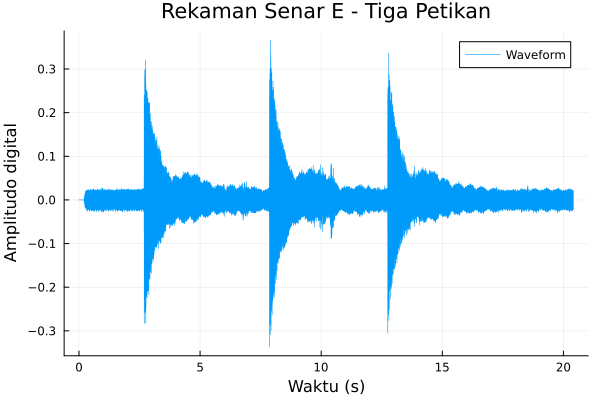
\includegraphics[width=0.5\textwidth]
            {../results/figures/waveform_rekaman.png}
            \caption{Bentuk gelombang sinyal audio hasil perekaman
            tiga petikan senar gitar.}
            \label{fig:waveform-rekaman}
        \end{figure}

    \subsection{Pengolahan Rekaman Audio}

        Rekaman audio terlebih dahulu dibagi menjadi tiga bagian yang masing-masing merepresentasikan satu petikan. 
        Posisi waktu setiap petikan ditentukan dengan mengamati perubahan nilai \textit{Root Mean Square} (RMS) sinyal menggunakan jendela waktu sebesar $10\,\mathrm{ms}$. 
        Puncak RMS digunakan sebagai acuan untuk memilih bagian sinyal yang akan dianalisis.

        Untuk setiap petikan, dipilih segmen berdurasi $1\,\mathrm{s}$ setelah puncak RMS terdeteksi. 
        Nilai rata-rata sinyal pada setiap segmen dikurangi untuk menghilangkan komponen DC. 
        Selanjutnya, sinyal dikalikan dengan fungsi jendela Hann sebelum dilakukan transformasi Fourier. 
        Penggunaan fungsi jendela bertujuan mengurangi kebocoran spektral (\textit{spectral leakage}) akibat pemotongan sinyal pada interval waktu terbatas \cite{Harris1978}.

        Transformasi Fourier diskret dihitung menggunakan FFT.
        Untuk jumlah sampel $N$, resolusi frekuensi nominal
        ditentukan oleh
        \begin{equation}
            \Delta f = \frac{f_s}{N}.
            \label{eq:frequency-resolution}
        \end{equation}
        Dengan durasi segmen sebesar $1\,\mathrm{s}$ dan $f_s=44{,}1\,\mathrm{kHz}$, diperoleh $N=44100$ sampel sehingga resolusi frekuensi nominal sebesar $\Delta f=1\,\mathrm{Hz}$.

    \subsection{Identifikasi Frekuensi Fundamental}

        Frekuensi fundamental ditentukan berdasarkan pola harmonik pada spektrum frekuensi. 
        Untuk senar ideal yang kedua ujungnya terikat, frekuensi harmonik memenuhi hubungan
        \begin{equation}
            f_n = n f_1,
            \qquad n=1,2,3,\ldots,
            \label{eq:harmonic-frequency}
        \end{equation}
        Oleh karena itu, identifikasi frekuensi fundamental tidak hanya didasarkan pada puncak spektrum dengan amplitudo terbesar, tetapi juga pada kesesuaian puncak-puncak lainnya terhadap kelipatan frekuensi tersebut.

        Hasil analisis menunjukkan adanya pola harmonik dengan frekuensi dasar sekitar $328{,}5\,\mathrm{Hz}$. 
        Estimasi frekuensi fundamental dari ketiga petikan ditampilkan pada Tabel~\ref{tab:fundamental-frequency}.
        \begin{table}[htbp]
            \centering
            \caption{Estimasi frekuensi fundamental dari tiga petikan.}
            \label{tab:fundamental-frequency}
            \begin{tabular}{ccc}
                \hline
                Petikan & Interval analisis (s) &
                $f_1$ (Hz) \\
                \hline
                1 & 2{,}780--3{,}780 & 328{,}512 \\
                2 & 7{,}960--8{,}960 & 328{,}516 \\
                3 & 12{,}830--13{,}830 & 328{,}475 \\
                \hline
                Rata-rata & -- & 328{,}501 \\
                \hline
            \end{tabular}
        \end{table}
        Estimasi frekuensi pada tabel diperoleh melalui interpolasi puncak spektrum di sekitar bin frekuensi maksimum.
        Rata-rata ketiga hasil pengukuran adalah $\bar{f}_1=328{,}501\,\mathrm{Hz}$ dengan simpangan baku sebesar $0{,}023\,\mathrm{Hz}$. 
        Nilai ini menunjukkan konsistensi hasil estimasi dari ketiga petikan.

        Namun, simpangan baku tersebut menggambarkan variasi antarpetikan, bukan resolusi frekuensi FFT.
        Resolusi frekuensi nominal tetap sebesar $1\,\mathrm{Hz}$.
        Dengan demikian, angka desimal pada hasil interpolasi digunakan untuk membandingkan estimasi puncak spektrum, dan tidak dapat langsung diartikan sebagai ketelitian absolut pengukuran.
        \begin{figure}[htbp]
            \centering
            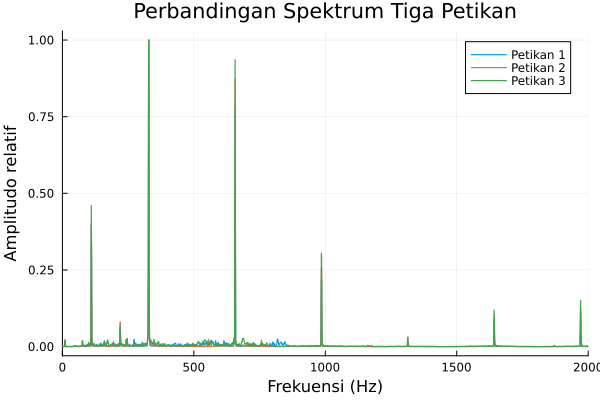
\includegraphics[width=0.5\textwidth]
            {../results/figures/perbandingan_FFT.png}
            \caption{Perbandingan spektrum frekuensi dari ketiga
            petikan senar gitar.}
            \label{fig:perbandingan-fft}
        \end{figure}
        Selain kelompok puncak harmonik yang berpusat pada frekuensi fundamental, spektrum juga menunjukkan komponen di sekitar $110\,\mathrm{Hz}$ dan kelipatannya. 
        Komponen tersebut tidak mengikuti pola harmonik dari $328{,}5\,\mathrm{Hz}$ sehingga tidak digunakan dalam penentuan frekuensi fundamental.
        Sumber komponen tersebut belum dapat dipastikan dari analisis rekaman ini.

\section{Metode Numerik}
\label{sec:metode-numerik}

    \subsection{Diskretisasi Persamaan Gelombang}

        Persamaan gelombang diselesaikan menggunakan metode beda hingga eksplisit dengan pendekatan beda pusat terhadap turunan ruang dan waktu \cite{LeVeque2007}. 
        Domain ruang dibagi menjadi $N_x$ interval dengan jarak antartitik $\Delta x=L/N_x$, sedangkan domain waktu didiskretisasi dengan langkah waktu $\Delta t$. Posisi dan waktu diskret dinyatakan sebagai
        \begin{equation}
            x_i=i\Delta x, \qquad t_n=n\Delta t,
        \end{equation}
        dengan $i=0,1,\ldots,N_x$ dan $n=0,1,\ldots,N_t$.
        Simpangan pada posisi $x_i$ dan waktu $t_n$ dituliskan sebagai $y_i^n$.

        Turunan kedua terhadap waktu dan ruang didekati dengan
        \begin{equation}
            \frac{\partial^2 y}{\partial t^2} \approx \frac{y_i^{n+1}-2y_i^n+y_i^{n-1}}{\Delta t^2},
        \end{equation}

        \begin{equation}
            \frac{\partial^2 y}{\partial x^2} \approx \frac{y_{i+1}^n-2y_i^n+y_{i-1}^n}{\Delta x^2}.
        \end{equation}

        Dengan mensubstitusikan pendekatan tersebut ke dalam Persamaan~\eqref{eq:wave-equation}, diperoleh skema numerik
        \begin{equation}
            y_i^{n+1} = 2y_i^n-y_i^{n-1} +r^2 \left( y_{i+1}^n-2y_i^n+y_{i-1}^n \right),
            \label{eq:fd-wave}
        \end{equation}
        dengan faktor Courant didefinisikan sebagai
        \begin{equation}
            r=\frac{c\Delta t}{\Delta x}.
            \label{eq:courant}
        \end{equation}
        Kondisi batas tetap diterapkan pada setiap langkah waktu dengan menetapkan
        \begin{equation}
            y_0^n=y_{N_x}^n=0.
        \end{equation}

    \subsection{Implementasi Kondisi Awal}

        Skema pada Persamaan~\eqref{eq:fd-wave} membutuhkan dua tingkat waktu awal, yaitu $y_i^0$ dan $y_i^1$. 
        Nilai $y_i^0$ diperoleh dari profil simpangan awal, sedangkan $y_i^1$ dihitung menggunakan ekspansi Taylor terhadap waktu,
        \begin{equation}
            y(x,\Delta t) = y(x,0) + \Delta t \left.\frac{\partial y}{\partial t}\right|_{t=0} + \frac{\Delta t^2}{2} \left.\frac{\partial^2 y}{\partial t^2}\right|_{t=0} + \mathcal{O}(\Delta t^3).
        \end{equation}
        Berdasarkan persamaan gelombang dan kondisi kecepatan awal nol, diperoleh pendekatan langkah waktu pertama
        \begin{equation}
            y_i^1 = y_i^0+ \frac{r^2}{2} \left( y_{i+1}^0-2y_i^0+y_{i-1}^0 \right).
            \label{eq:first-time-step}
        \end{equation}
        Persamaan~\eqref{eq:first-time-step} digunakan untuk menginisialisasi simulasi sebelum skema beda hingga dijalankan secara iteratif.

    \subsection{Analisis Kestabilan dan Dispersi Numerik}

        Kestabilan skema beda hingga dianalisis menggunakan pendekatan Fourier dengan mengasumsikan solusi berbentuk gelombang diskret
        \begin{equation}
            y_i^n=G^n e^{\mathrm{i}k x_i},
        \end{equation}
        dengan $G$ merupakan faktor amplifikasi dan $k$ adalah bilangan gelombang.
        Substitusi bentuk tersebut ke dalam Persamaan~\eqref{eq:fd-wave} menghasilkan
        \begin{equation}
            G^2 - 2\left[ 1-2r^2\sin^2\left(\frac{k\Delta x}{2}\right) \right] G+1=0.
        \end{equation}
        Dengan menyatakan $G=e^{-\mathrm{i}\omega_{\mathrm{num}} \Delta t}$, diperoleh relasi dispersi numerik
        \begin{equation}
            \sin^2 \left( \frac{\omega_{\mathrm{num}}\Delta t}{2} \right) = r^2\sin^2\left(\frac{k\Delta x}{2}\right),
            \label{eq:numerical-dispersion}
        \end{equation}
        dengan $\omega_{\mathrm{num}}$ merupakan frekuensi sudut numerik. 
        Agar faktor amplifikasi tidak bertambah tanpa batas, syarat kestabilan skema adalah
        \begin{equation}
            0\leq r\leq 1.
            \label{eq:cfl-condition}
        \end{equation}
        Relasi dispersi pada Persamaan~\eqref{eq:numerical-dispersion} juga menunjukkan bahwa kecepatan fase numerik dapat berbeda dari kecepatan fase gelombang kontinu. 
        Untuk $r=1$, skema ini tidak mengalami dispersi fase pada rentang bilangan gelombang yang terwakili oleh grid.
        Sebaliknya, untuk $r<1$, kecepatan fase numerik bergantung pada bilangan gelombang sehingga dapat terjadi dispersi numerik.

        Pengujian kestabilan dilakukan dengan menggunakan $N_x=100$ dan tiga variasi faktor Courant, yaitu $r=0{,}80$, $r=1{,}00$, dan $r=1{,}05$. 
        Simulasi dijalankan hingga waktu sekitar $2L/c$ dengan pengamatan profil gelombang pada waktu $L/(2c)$ dan $L/c$.
        Untuk mendeteksi pertumbuhan solusi yang tidak stabil, amplitudo maksimum dipantau pada setiap langkah waktu.
        Simulasi dihentikan apabila nilai simpangan mencapai $10^6h$ atau menghasilkan nilai yang tidak hingga (\textit{non-finite}).

    \subsection{Pengujian Konvergensi Numerik}

        Konvergensi metode diuji menggunakan profil awal berbentuk sinus yang memiliki solusi analitik
        \begin{equation}
            y_{\mathrm{eksak}}(x,t) = h\sin\left(\frac{\pi x}{L}\right) \cos\left(\frac{\pi c t}{L}\right).
            \label{eq:analytical-solution}
        \end{equation}
        Profil ini memenuhi kondisi batas tetap dan kondisi kecepatan awal nol. 
        Simulasi dilakukan dengan faktor Courant $r=0{,}80$ serta variasi jumlah interval $N_x=50$, $100$, dan $200$. 
        Perbandingan dilakukan pada waktu fisik yang sama, yaitu
        \begin{equation}
            t^*=\frac{0{,}8L}{c}.
        \end{equation}
        Pemilihan waktu tersebut memungkinkan evaluasi dilakukan tepat pada langkah waktu ke-$N_x$ untuk setiap ukuran grid yang digunakan.

        Galat solusi dihitung menggunakan \textit{Root Mean Square Error} (RMSE),
        \begin{equation}
            E_{N_x}. = \sqrt{ \frac{1}{N_x+1} \sum_{i=0}^{N_x} \left[ y_i^{\mathrm{num}}(t^*) - y_{\mathrm{eksak}}(x_i,t^*)\right]^2},
            \label{eq:rmse}
        \end{equation}
        dengan $y_i^{\mathrm{num}}$ merupakan solusi numerik.
        Orde konvergensi dihitung melalui perbandingan galat pada dua ukuran grid yang berurutan,
        \begin{equation}
            p = \frac{ \ln(E_{N_x}/E_{2N_x}) }{\ln 2}.
            \label{eq:convergence-order}
        \end{equation}

    \subsection{Diskretisasi Persamaan Gelombang Teredam}

        Untuk menganalisis pengaruh redaman, persamaan gelombang teredam pada Persamaan~\eqref{eq:damped-wave-equation} didiskretisasi menggunakan pendekatan beda pusat yang sama. 
        Turunan pertama terhadap waktu didekati dengan
        \begin{equation}
            \frac{\partial y}{\partial t} \approx \frac{y_i^{n+1}-y_i^{n-1}}{2\Delta t}.
        \end{equation}
        Dengan mendefinisikan
        \begin{equation}
            q=\frac{\gamma\Delta t}{2},
        \end{equation}
        skema numerik gelombang teredam diperoleh sebagai
        \begin{equation}
            (1+q)y_i^{n+1} = 2y_i^n +r^2 \left( y_{i+1}^n-2y_i^n+y_{i-1}^n \right) -(1-q)y_i^{n-1}.
            \label{eq:fd-damped}
        \end{equation}

        Apabila $\gamma=0$, maka $q=0$ dan Persamaan~\eqref{eq:fd-damped} kembali menjadi skema persamaan gelombang tanpa redaman. 
        Kondisi awal kecepatan nol juga menghasilkan persamaan inisialisasi gan Persamaan~\eqref{eq:first-time-step}.

        Pengaruh redaman diamati melalui perbandingan dua kondisi, yaitu $\gamma=0$ dan $\gamma=15\,\mathrm{s}^{-1}$.
        Kedua simulasi menggunakan $N_x=100$, $r=0{,}80$, dan durasi simulasi sebesar $0{,}2\,\mathrm{s}$.

    \subsection{Perhitungan Energi Sistem}

        Energi mekanik kontinu pada senar didefinisikan sebagai jumlah energi kinetik dan energi potensial,
        \begin{equation}
            E(t)= \frac{\mu}{2} \int_0^L \left(\frac{\partial y}{\partial t}\right)^2 dx + \frac{T}{2} \int_0^L \left(\frac{\partial y}{\partial x}\right)^2 dx.
            \label{eq:continuous-energy}
        \end{equation}
        Dengan menggunakan persamaan gelombang teredam dan kondisi batas tetap, laju perubahan energi memenuhi
        \begin{equation}
            \frac{dE}{dt} = -\mu\gamma \int_0^L \left(\frac{\partial y}{\partial t}\right)^2 dx \leq 0.
            \label{eq:energy-dissipation}
        \end{equation}

        Persamaan~\eqref{eq:energy-dissipation} menunjukkan bahwa energi sistem tidak bertambah untuk $\gamma\geq0$.
        Pada kondisi tanpa redaman, energi kontinu bersifat konstan, sedangkan pada kondisi dengan redaman energi berkurang terhadap waktu.

        Dalam perhitungan numerik, kecepatan transversal didekati menggunakan beda pusat terhadap waktu,
        \begin{equation}
            v_i^n= \frac{y_i^{n+1}-y_i^{n-1}}{2\Delta t}.
        \end{equation}
        Untuk waktu awal digunakan kondisi $v_i^0=0$, sedangkan pada waktu akhir digunakan beda mundur.
        Turunan ruang dihitung menggunakan beda maju,
        \begin{equation}
            \left(\frac{\partial y}{\partial x}\right)_i^n
            \approx
            \frac{y_{i+1}^n-y_i^n}{\Delta x}.
        \end{equation}
        Energi kinetik dihitung menggunakan integrasi trapesium, sedangkan energi potensial dihitung dengan penjumlahan kontribusi setiap interval grid. 
        Dengan demikian, pendekatan energi diskret dinyatakan sebagai
        \begin{equation}
            E_{\mathrm{num}}^n = \frac{\mu}{2} \operatorname{Trapz}_x\left[(v_i^n)^2\right] + \frac{T}{2}\Delta x \sum_{i=0}^{N_x-1} \left( \frac{y_{i+1}^n-y_i^n}{\Delta x} \right)^2.
            \label{eq:discrete-energy}
        \end{equation}

        Untuk membandingkan perubahan energi terhadap waktu, digunakan energi ternormalisasi
        \begin{equation}
            \widehat{E}(t_n) = \frac{E_{\mathrm{num}}^n}{E_{\mathrm{num}}^0}.
            \label{eq:normalized-energy}
        \end{equation}
        Konvergensi perhitungan energi diuji pada kondisi tanpa redaman menggunakan variasi $N_x=50$, $100$, dan $200$, dengan faktor Courant $r=0{,}80$ dan
        durasi simulasi $0{,}2\,\mathrm{s}$. 
        Penyimpangan energi ternormalisasi terhadap nilai awal dievaluasi menggunakan simpangan maksimum dan RMSE terhadap waktu, sehingga pengaruh ukuran grid terhadap akurasi perhitungan energi dapat dianalisis.

    \subsection{Implementasi Komputasi}

        Seluruh simulasi numerik diimplementasikan menggunakan bahasa pemrograman Julia versi $1.13.3$. 
        Paket yang digunakan meliputi FFTW versi $1.10.0$ untuk transformasi
        Fourier, Plots versi $1.41.7$ untuk visualisasi hasil, dan WAV versi $1.2.0$ untuk pembacaan rekaman audio.
        Pustaka standar Statistics dan Printf juga digunakan dalam pengolahan data dan penyajian hasil.

        Kode program disusun dalam beberapa berkas terpisah berdasarkan tahapan analisis, meliputi pengolahan audio, estimasi parameter fisis, simulasi gelombang, pengujian kestabilan, pengujian konvergensi, dan analisis energi.
        Hasil komputasi disimpan dalam format CSV, sedangkan grafik dan animasi disimpan dalam format PNG dan GIF.
        Lingkungan komputasi didefinisikan melalui berkas \texttt{Project.toml} dan \texttt{Manifest.toml} untuk menjaga konsistensi versi paket yang digunakan.

\section{Hasil dan Pembahasan}
\label{sec:hasil-pembahasan}

\subsection{Pengujian Kestabilan CFL}

Pengujian kestabilan dilakukan menggunakan jumlah interval
ruang $N_x=100$ dengan tiga variasi faktor Courant, yaitu
$r=0{,}80$, $r=1{,}00$, dan $r=1{,}05$. Panjang domain
dan parameter fisis dibuat tetap sehingga variasi langkah
waktu ditentukan oleh perubahan nilai faktor Courant.
Ringkasan parameter dan hasil simulasi ditampilkan pada
Tabel~\ref{tab:cfl-results}.

\begin{table}[htbp]
    \centering
    \caption{Hasil pengujian kestabilan untuk berbagai faktor Courant.}
    \label{tab:cfl-results}
    \begin{tabular}{ccccc}
        \hline
        $r$ & $\Delta x$ (m) & $\Delta t$ (s) &
        Jumlah langkah & Hasil \\
        \hline
        0{,}80 & 0{,}00658 &
        $1{,}2177\times10^{-5}$ & 250 & Stabil \\

        1{,}00 & 0{,}00658 &
        $1{,}5221\times10^{-5}$ & 200 & Stabil \\

        1{,}05 & 0{,}00658 &
        $1{,}5982\times10^{-5}$ & 35 &
        Tidak stabil \\
        \hline
    \end{tabular}
\end{table}

Pada $r=0{,}80$ dan $r=1{,}00$, simulasi dapat
diselesaikan hingga waktu sekitar $2L/c$ tanpa menunjukkan
pertumbuhan amplitudo yang tidak terkendali. Amplitudo
maksimum tetap berada di sekitar amplitudo awal,
yaitu $10^{-3}\,\mathrm{m}$. Hasil ini sesuai dengan
syarat kestabilan $r\leq1$ pada skema yang digunakan.

Sebaliknya, pada $r=1{,}05$, amplitudo solusi meningkat
secara signifikan sehingga simulasi dihentikan setelah
35 langkah waktu. Waktu penghentian tercatat sekitar
$5{,}59\times10^{-4}\,\mathrm{s}$, sebelum mencapai
waktu pengamatan $L/(2c)$ maupun $L/c$. Amplitudo pada
langkah penghentian mencapai sekitar
$1{,}522\times10^3\,\mathrm{m}$, melampaui ambang
penghentian sebesar $10^6h=10^3\,\mathrm{m}$.
Nilai tersebut merupakan hasil pemeriksaan setelah
pembaruan langkah waktu sehingga dapat sedikit melampaui
ambang yang ditentukan.

Perkembangan amplitudo maksimum selama simulasi
ditunjukkan pada Gambar~\ref{fig:cfl-amplitude}.
Hasil tersebut memperlihatkan perbedaan yang jelas antara
solusi stabil dan solusi tidak stabil ketika faktor
Courant melampaui batas kestabilan.

\begin{figure}[htbp]
    \centering
    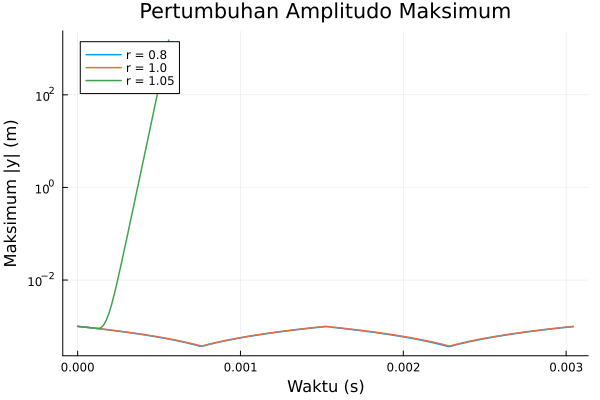
\includegraphics[width=0.5\textwidth]
    {../results/figures/cfl_max_amplitude.png}
    \caption{Perkembangan amplitudo maksimum terhadap waktu
    untuk variasi faktor Courant.}
    \label{fig:cfl-amplitude}
\end{figure}

Perbandingan profil gelombang pada waktu fisik yang sama
ditampilkan pada Gambar~\ref{fig:cfl-profile-half}
dan Gambar~\ref{fig:cfl-profile-full}. Kedua gambar
memperlihatkan hasil untuk kasus stabil. Kasus
$r=1{,}05$ tidak ditampilkan karena simulasi telah
dihentikan sebelum mencapai waktu pengamatan.

\begin{figure}[htbp]
    \centering
    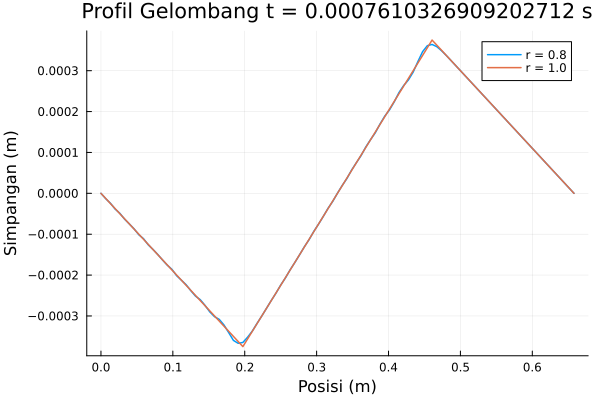
\includegraphics[width=0.5\textwidth]
    {../results/figures/cfl_profile_L_2c.png}
    \caption{Perbandingan profil gelombang pada waktu
    $t=L/(2c)$ untuk kasus stabil.}
    \label{fig:cfl-profile-half}
\end{figure}

\begin{figure}[htbp]
    \centering
    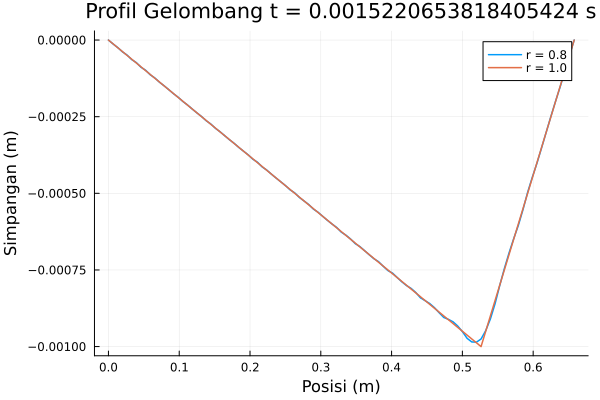
\includegraphics[width=0.5\textwidth]
    {../results/figures/cfl_profile_L_c.png}
    \caption{Perbandingan profil gelombang pada waktu
    $t=L/c$ untuk kasus stabil.}
    \label{fig:cfl-profile-full}
\end{figure}

Hasil pengujian menunjukkan bahwa pemilihan langkah
waktu memiliki pengaruh langsung terhadap kestabilan
solusi numerik. Selain kestabilan, faktor Courant juga
memengaruhi dispersi numerik. Untuk $r=1$, skema beda
hingga yang digunakan memiliki relasi dispersi yang
sesuai dengan gelombang kontinu pada mode yang
terwakili grid. Sementara itu, untuk $r=0{,}80$,
perbedaan kecepatan fase numerik terhadap solusi kontinu
dapat menyebabkan perubahan bentuk profil gelombang
selama perambatan.

\subsection{Pengujian Konvergensi Solusi Gelombang}

Pengujian konvergensi dilakukan dengan membandingkan
solusi numerik terhadap solusi analitik berbentuk
sinus pada Persamaan~\eqref{eq:analytical-solution}.
Simulasi menggunakan faktor Courant $r=0{,}80$ dengan
variasi jumlah interval $N_x=50$, $100$, dan $200$.
Perbandingan dilakukan pada waktu fisik yang sama,
yaitu $t^*=0{,}8L/c$.

Waktu tersebut dipilih karena dapat dicapai tepat pada
langkah waktu ke-$N_x$ untuk setiap ukuran grid yang
digunakan. Dengan demikian, perbandingan galat tidak
dipengaruhi oleh perbedaan pembulatan jumlah langkah
waktu. Hasil perhitungan galat ditampilkan pada
Tabel~\ref{tab:convergence-results}.

\begin{table}[htbp]
    \centering
    \caption{Hasil pengujian konvergensi solusi gelombang.}
    \label{tab:convergence-results}
    \begin{tabular}{ccccc}
        \hline
        $N_x$ & $\Delta x$ (m) & $\Delta t$ (s) &
        Jumlah langkah & RMSE (m) \\
        \hline
        50 & 0{,}01316 &
        $2{,}4353\times10^{-5}$ & 50 &
        $6{,}1269\times10^{-8}$ \\

        100 & 0{,}00658 &
        $1{,}2177\times10^{-5}$ & 100 &
        $1{,}5389\times10^{-8}$ \\

        200 & 0{,}00329 &
        $6{,}0883\times10^{-6}$ & 200 &
        $3{,}8566\times10^{-9}$ \\
        \hline
    \end{tabular}
\end{table}

Berdasarkan tabel tersebut, nilai RMSE mengalami
penurunan ketika jumlah interval grid diperbesar.
Ketika $N_x$ dinaikkan dari 50 menjadi 100, galat
berkurang dari sekitar $6{,}13\times10^{-8}\,\mathrm{m}$
menjadi $1{,}54\times10^{-8}\,\mathrm{m}$. Peningkatan
jumlah interval menjadi 200 kembali menurunkan galat
hingga sekitar $3{,}86\times10^{-9}\,\mathrm{m}$.

Orde konvergensi yang diperoleh dari perbandingan
galat dua ukuran grid berurutan adalah

\begin{align}
    p_{50\rightarrow100} &= 1{,}9933,\\
    p_{100\rightarrow200} &= 1{,}9965.
\end{align}

Rata-rata orde konvergensi yang diperoleh mendekati
dua. Hasil tersebut konsisten dengan ketelitian
orde kedua dari pendekatan beda pusat terhadap
ruang dan waktu yang digunakan dalam skema numerik.

Perbandingan profil solusi numerik dan analitik
ditampilkan pada Gambar~\ref{fig:convergence-profile},
sedangkan penurunan galat terhadap ukuran grid
ditampilkan pada Gambar~\ref{fig:convergence-error}.

\begin{figure}[htbp]
    \centering
    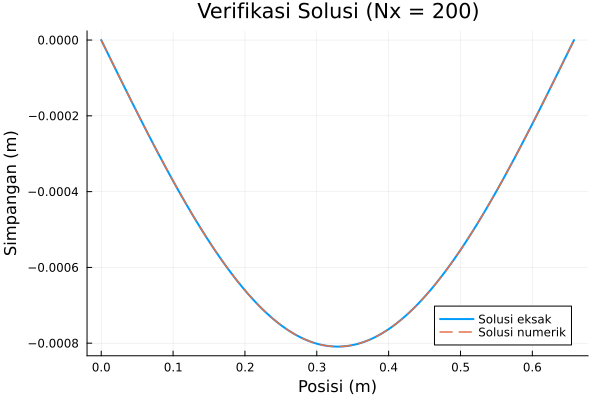
\includegraphics[width=0.5\textwidth]
    {../results/figures/convergence_profile.png}
    \caption{Perbandingan profil solusi numerik dan
    solusi analitik pada beberapa ukuran grid.}
    \label{fig:convergence-profile}
\end{figure}

\begin{figure}[htbp]
    \centering
    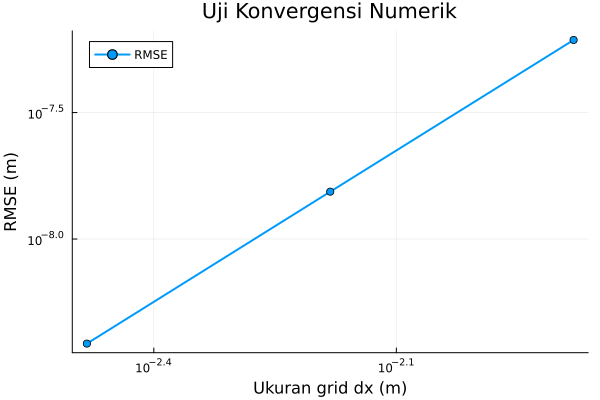
\includegraphics[width=0.5\textwidth]
    {../results/figures/convergence_error.png}
    \caption{Perubahan RMSE terhadap jumlah interval grid
    pada pengujian konvergensi.}
    \label{fig:convergence-error}
\end{figure}

\subsection{Pengaruh Redaman terhadap Evolusi Gelombang}

Pengaruh redaman dianalisis dengan membandingkan
dua kondisi, yaitu tanpa redaman ($\gamma=0$)
dan dengan redaman $\gamma=15\,\mathrm{s}^{-1}$.
Kedua simulasi menggunakan jumlah interval
$N_x=100$, faktor Courant $r=0{,}80$, dan
durasi simulasi sekitar $0{,}2\,\mathrm{s}$.
Langkah waktu yang digunakan adalah
$1{,}2177\times10^{-5}\,\mathrm{s}$ dengan
jumlah langkah waktu sebanyak 16426.

Profil gelombang pada kondisi tanpa redaman
memperlihatkan osilasi yang tetap berlangsung
selama simulasi. Sebaliknya, pada kondisi dengan
redaman, amplitudo gelombang berkurang terhadap
waktu. Perbandingan profil gelombang tersebut
ditampilkan pada Gambar~\ref{fig:damped-profile}.

\begin{figure}[htbp]
    \centering
    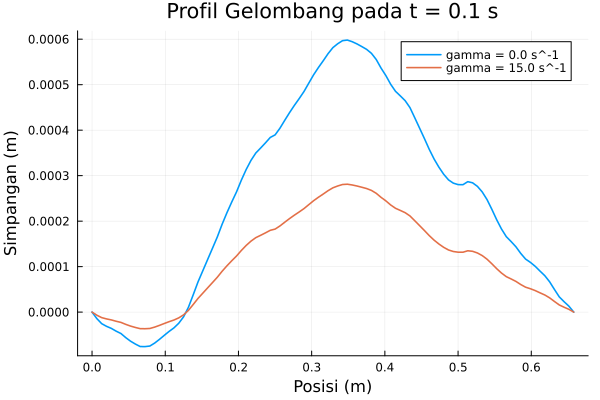
\includegraphics[width=0.5\textwidth]
    {../results/figures/damped_profile.png}
    \caption{Perbandingan profil gelombang pada kondisi
    tanpa redaman dan dengan redaman.}
    \label{fig:damped-profile}
\end{figure}

Perubahan profil gelombang juga divisualisasikan
melalui animasi hasil simulasi. Berkas animasi
\texttt{damped\_comparison.gif} disertakan sebagai
keluaran komputasi pendukung. Visualisasi tersebut
memperlihatkan bahwa penambahan suku redaman
mengurangi amplitudo osilasi seiring bertambahnya
waktu simulasi.

\subsection{Analisis Energi Sistem}

Perubahan energi sistem dianalisis dengan menggunakan
energi ternormalisasi terhadap energi awal,
$\widehat{E}(t)=E(t)/E(0)$. Hasil perhitungan
menunjukkan bahwa energi pada kondisi tanpa redaman
mengalami fluktuasi kecil di sekitar nilai awal.
Pada akhir simulasi, rasio energi terhadap energi awal
adalah sekitar $0{,}99699$, dengan nilai minimum
sekitar $0{,}99323$.

Pada kondisi dengan redaman, energi mengalami
penurunan yang lebih besar. Rasio energi pada akhir
simulasi mencapai sekitar $0{,}04966$, yang berarti
energi numerik tersisa sekitar $4{,}97\%$ dari
energi awal. Perbandingan hasil perhitungan energi
ditampilkan pada Gambar~\ref{fig:damped-energy}.

\begin{table}[htbp]
    \centering
    \caption{Perbandingan energi numerik pada kondisi
    tanpa redaman dan dengan redaman.}
    \label{tab:damped-energy}
    \begin{tabular}{cccc}
        \hline
        $\gamma$ ($\mathrm{s}^{-1}$) &
        $E(0)$ (J) &
        $E(t_{\mathrm{akhir}})$ (J) &
        $\widehat{E}(t_{\mathrm{akhir}})$ \\
        \hline
        0 & $3{,}0351\times10^{-2}$ &
        $3{,}0259\times10^{-2}$ & 0{,}99699 \\

        15 & $3{,}0351\times10^{-2}$ &
        $1{,}5072\times10^{-3}$ & 0{,}04966 \\
        \hline
    \end{tabular}
\end{table}

\begin{figure}[htbp]
    \centering
    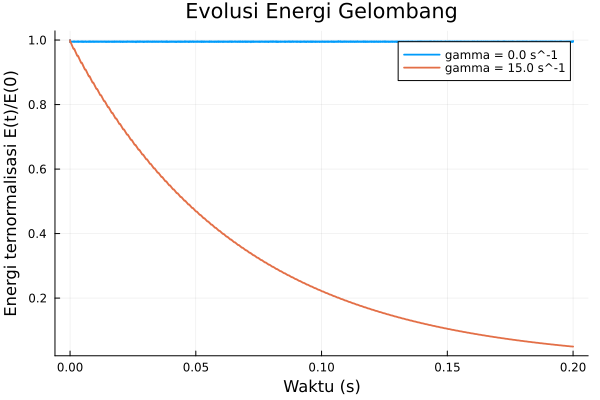
\includegraphics[width=0.5\textwidth]
    {../results/figures/damped_energy.png}
    \caption{Perubahan energi ternormalisasi terhadap
    waktu untuk beberapa nilai koefisien redaman.}
    \label{fig:damped-energy}
\end{figure}

Pada kondisi $\gamma=0$, persamaan energi kontinu
menyatakan bahwa energi mekanik seharusnya konstan.
Fluktuasi kecil yang diperoleh dari perhitungan numerik
menunjukkan adanya penyimpangan akibat pendekatan
diskret pada turunan dan integrasi energi. Oleh sebab
itu, perubahan energi pada kasus ini tidak dapat
langsung diinterpretasikan sebagai redaman fisis.

Sebaliknya, penurunan energi yang besar pada
$\gamma=15\,\mathrm{s}^{-1}$ sesuai dengan keberadaan
suku disipatif pada persamaan gelombang teredam.
Hasil tersebut menunjukkan bahwa redaman memindahkan
energi mekanik keluar dari sistem yang dimodelkan,
sehingga amplitudo gelombang dan energi total
berkurang terhadap waktu.

\subsection{Konvergensi Perhitungan Energi}

Konvergensi perhitungan energi diuji pada kondisi
tanpa redaman dengan membandingkan tiga ukuran grid,
yaitu $N_x=50$, $100$, dan $200$. Faktor Courant
dipertahankan sebesar $r=0{,}80$ dan durasi simulasi
sebesar $0{,}2\,\mathrm{s}$. Penyimpangan energi
dianalisis melalui simpangan maksimum dan RMSE
energi ternormalisasi terhadap nilai awal.

Hasil pengujian ditampilkan pada
Tabel~\ref{tab:energy-convergence}.

\begin{table}[htbp]
    \centering
    \caption{Hasil pengujian konvergensi perhitungan energi
    pada kondisi tanpa redaman.}
    \label{tab:energy-convergence}
    \begin{tabular}{cccc}
        \hline
        $N_x$ &
        Simpangan maksimum &
        RMSE &
        $\widehat{E}(t_{\mathrm{akhir}})$ \\
        \hline
        50 & 0{,}01484 & 0{,}01008 & 0{,}99864 \\
        100 & 0{,}00677 & 0{,}00502 & 0{,}99492 \\
        200 & 0{,}00333 & 0{,}00250 & 0{,}99775 \\
        \hline
    \end{tabular}
\end{table}

Simpangan maksimum dan RMSE mengalami penurunan
secara konsisten ketika ukuran grid diperhalus.
Nilai RMSE berkurang dari sekitar $1{,}01\times10^{-2}$
pada $N_x=50$ menjadi $2{,}50\times10^{-3}$ pada
$N_x=200$. Hasil ini menunjukkan bahwa penyimpangan
perhitungan energi terhadap nilai awal semakin kecil
ketika resolusi grid ditingkatkan.

Nilai energi pada akhir simulasi tidak menunjukkan
penurunan yang monoton terhadap ukuran grid. Hal ini
menunjukkan bahwa evaluasi konvergensi energi tidak
cukup dilakukan hanya dengan membandingkan nilai
energi pada satu waktu akhir. Penggunaan simpangan
maksimum dan RMSE selama keseluruhan simulasi
memberikan gambaran yang lebih menyeluruh terhadap
perubahan energi numerik.

Simpangan maksimum dan RMSE energi ternormalisasi
terhadap ukuran grid ditampilkan pada
Gambar~\ref{fig:energy-convergence}. Sementara itu,
evolusi energi ternormalisasi terhadap waktu untuk
beberapa ukuran grid ditampilkan pada
Gambar~\ref{fig:energy-grid-comparison}.

\begin{figure}[htbp]
    \centering
    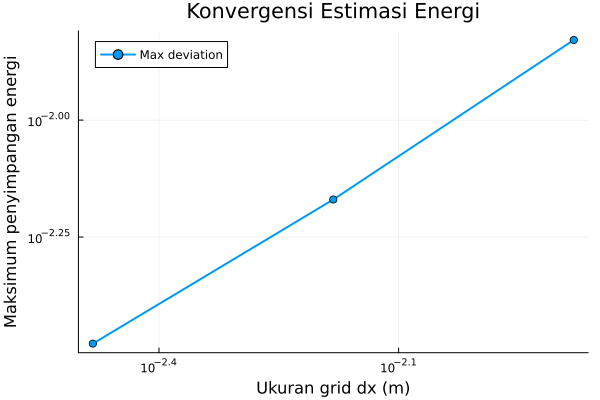
\includegraphics[width=0.5\textwidth]
    {../results/figures/energy_convergence.png}
    \caption{Simpangan maksimum energi ternormalisasi
    terhadap ukuran grid pada kondisi tanpa redaman.}
    \label{fig:energy-convergence}
\end{figure}

\begin{figure}[htbp]
    \centering
    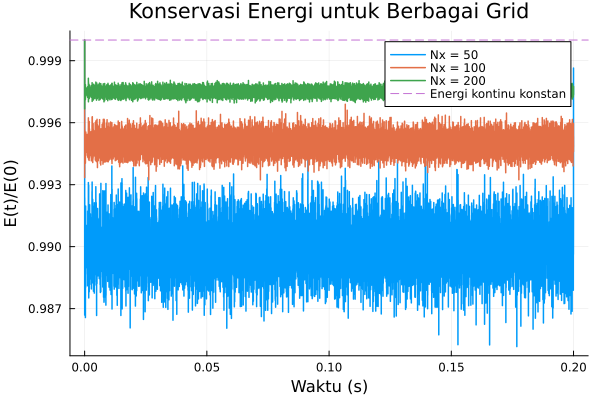
\includegraphics[width=0.5\textwidth]
    {../results/figures/energy_grid_comparison.png}
    \caption{Evolusi energi ternormalisasi terhadap waktu
    untuk beberapa ukuran grid pada kondisi tanpa redaman.}
    \label{fig:energy-grid-comparison}
\end{figure}

\section{Diskusi dan Keterbatasan Model}
\label{sec:diskusi}

\subsection{Interpretasi Estimasi Parameter Fisis}

Estimasi parameter fisis senar diperoleh dengan
menggabungkan hasil pengukuran panjang senar dan
frekuensi fundamental dengan asumsi massa senar.
Nilai cepat rambat gelombang dan tegangan yang diperoleh
bergantung langsung pada ketepatan parameter tersebut.
Khususnya, massa senar sebesar $22{,}5\,\mathrm{g}$
tidak diperoleh melalui pengukuran langsung, melainkan
diasumsikan berada pada rentang $22$--$23\,\mathrm{g}$.

Dengan mensubstitusikan $\mu=m/L$ ke dalam persamaan
tegangan, diperoleh

\begin{equation}
    T=4mLf_1^2.
\end{equation}

Hubungan tersebut menunjukkan bahwa estimasi tegangan
bergantung secara linear terhadap massa dan panjang
senar, serta secara kuadratik terhadap frekuensi
fundamental. Oleh karena itu, ketidakpastian massa
memberikan kontribusi dominan terhadap ketidakpastian
estimasi tegangan dalam perhitungan ini.

Nilai tegangan yang diperoleh, yaitu sekitar
$6{,}391\times10^3\,\mathrm{N}$, perlu ditafsirkan
secara hati-hati karena bergantung pada asumsi massa
yang digunakan. Dengan demikian, nilai tersebut
merupakan estimasi berdasarkan parameter masukan
yang diasumsikan, bukan hasil pengukuran tegangan
senar secara langsung. Pengukuran massa senar dan
tegangan aktual diperlukan untuk memperoleh estimasi
yang lebih representatif.

\subsection{Keterbatasan Pengukuran Eksperimen}

Analisis frekuensi dilakukan menggunakan rekaman
suara yang diperoleh dari mikrofon. Dengan demikian,
sinyal yang dianalisis merupakan tekanan akustik
yang dihasilkan oleh sistem senar dan badan gitar,
bukan pengukuran langsung terhadap simpangan
transversal senar. Karakteristik badan gitar,
ruangan, serta posisi mikrofon dapat memengaruhi
spektrum frekuensi yang terekam.

Selain itu, resolusi frekuensi nominal FFT yang
digunakan adalah $1\,\mathrm{Hz}$. Interpolasi
puncak spektrum menghasilkan estimasi frekuensi
dengan angka desimal, tetapi angka tersebut tidak
secara langsung menunjukkan ketelitian absolut
pengukuran. Variasi antarpetikan hanya memberikan
informasi mengenai konsistensi hasil estimasi dari
pengulangan eksperimen.

Spektrum juga menunjukkan komponen frekuensi di
sekitar $110\,\mathrm{Hz}$ yang tidak mengikuti
pola harmonik fundamental senar yang dianalisis.
Karena sumber komponen tersebut belum dapat
diidentifikasi secara pasti, komponen tersebut
tidak digunakan dalam penentuan frekuensi
fundamental.

\subsection{Keterbatasan Model Gelombang}

Model gelombang yang digunakan mengasumsikan senar
homogen dengan massa jenis linear dan tegangan
konstan, serta kedua ujung senar terikat sempurna.
Pendekatan ini mengabaikan beberapa karakteristik
senar nyata, seperti kekakuan lentur, ketidakseragaman
material, dan interaksi mekanik antara senar dengan
badan gitar. Karakteristik tersebut dapat memengaruhi
frekuensi harmonik dan respons akustik instrumen
\cite{FletcherRossing1998}.

Model gelombang tanpa redaman juga mengasumsikan
bahwa energi mekanik sistem tetap konstan.
Untuk merepresentasikan kehilangan energi, model
diperluas dengan menambahkan suku redaman linear
yang sebanding dengan kecepatan transversal.
Meskipun demikian, penggunaan satu koefisien redaman
konstan belum mencakup seluruh mekanisme disipasi
energi pada senar gitar yang sebenarnya.

Nilai $\gamma=15\,\mathrm{s}^{-1}$ dalam simulasi
digunakan sebagai parameter pembanding untuk
mengamati pengaruh redaman. Nilai tersebut tidak
diperoleh melalui pengukuran eksperimen, sehingga
hasil simulasi teredam tidak dimaksudkan sebagai
identifikasi kuantitatif redaman aktual senar gitar.

\subsection{Keterbatasan Metode Numerik dan
Perhitungan Energi}

Metode beda hingga eksplisit yang digunakan memiliki
batas kestabilan yang ditentukan oleh faktor Courant.
Hasil pengujian menunjukkan bahwa solusi stabil
ketika $r\leq1$, sedangkan penggunaan $r=1{,}05$
menghasilkan pertumbuhan amplitudo yang tidak
terkendali. Selain kestabilan, diskretisasi ruang
dan waktu juga dapat menimbulkan dispersi numerik
yang memengaruhi bentuk gelombang selama perambatan.

Pengujian konvergensi dengan profil sinus menunjukkan
bahwa skema numerik memiliki orde konvergensi
mendekati dua. Namun, hasil tersebut diperoleh dari
profil awal yang mulus dan memiliki solusi analitik.
Profil awal segitiga yang digunakan pada simulasi
senar memiliki perubahan kemiringan yang tidak
kontinu pada posisi petikan. Oleh karena itu,
keberadaan komponen gelombang berfrekuensi tinggi
dapat membuat respons numeriknya berbeda dari
pengujian konvergensi dengan profil sinus.

Perhitungan energi juga menggunakan pendekatan
diskret terhadap kecepatan, gradien ruang, dan
integrasi spasial. Hal ini menyebabkan energi
numerik pada kondisi tanpa redaman tidak selalu
konstan, meskipun energi kontinu secara teoritis
tetap terjaga. Pengujian dengan beberapa ukuran
grid menunjukkan bahwa penyimpangan energi
berkurang ketika resolusi grid ditingkatkan.
Dengan demikian, perubahan energi pada simulasi
numerik perlu diinterpretasikan dengan
mempertimbangkan galat diskretisasi yang digunakan.

\section{Kesimpulan}
\label{sec:kesimpulan}

Berdasarkan pengukuran eksperimen dan simulasi numerik
yang telah dilakukan, diperoleh beberapa kesimpulan
sebagai berikut.

\begin{enumerate}
    \item Analisis spektrum audio dari tiga petikan senar
    menghasilkan estimasi frekuensi fundamental rata-rata
    sebesar $328{,}501\,\mathrm{Hz}$. Dengan panjang senar
    sebesar $0{,}658\,\mathrm{m}$ dan asumsi massa
    $22{,}5\,\mathrm{g}$, diperoleh estimasi massa jenis
    linear sebesar $0{,}03419\,\mathrm{kg/m}$,
    cepat rambat gelombang sebesar $432{,}31\,\mathrm{m/s}$,
    dan tegangan sebesar $6{,}391\times10^3\,\mathrm{N}$.
    Nilai parameter tersebut bergantung pada asumsi massa
    senar yang digunakan.

    \item Metode beda hingga eksplisit berhasil
    diimplementasikan untuk menyelesaikan persamaan
    gelombang satu dimensi. Pengujian kestabilan
    menunjukkan bahwa simulasi stabil untuk
    $r=0{,}80$ dan $r=1{,}00$, sedangkan
    $r=1{,}05$ menghasilkan pertumbuhan amplitudo
    yang tidak terkendali. Pengujian konvergensi
    menggunakan solusi analitik menghasilkan orde
    konvergensi rata-rata sekitar $1{,}995$, yang
    mendekati orde kedua sesuai dengan skema numerik
    yang digunakan.

    \item Penambahan suku redaman dengan
    $\gamma=15\,\mathrm{s}^{-1}$ menghasilkan penurunan
    amplitudo dan energi gelombang yang signifikan.
    Pada akhir simulasi, energi ternormalisasi tersisa
    sekitar $4{,}97\%$ dari energi awal, sedangkan pada
    kondisi tanpa redaman nilainya sekitar $99{,}70\%$.
    Pengujian konvergensi energi tanpa redaman juga
    menunjukkan bahwa penyimpangan energi numerik
    berkurang ketika ukuran grid diperhalus.
\end{enumerate}

Secara keseluruhan, hasil pekerjaan menunjukkan bahwa
metode beda hingga dapat digunakan untuk mempelajari
evolusi gelombang pada senar melalui pengujian
kestabilan, konvergensi, dan pengaruh redaman.
Namun, interpretasi parameter fisis dan hasil simulasi
tetap perlu mempertimbangkan asumsi serta keterbatasan
model yang digunakan.

\section*{Pernyataan Penggunaan AI}



\section*{Daftar Pustaka}

\bibliography{reference}



\end{document}